\sloppy

Les ambitions de la mission Défense et Sécurité sont aujourd’hui implémentées à travers un centre d’excellence dédié au domaine de la Sécurité et Défense afin de faciliter le développement et le transfert à court, moyen et long terme de technologies issues de la Recherche.

Ce chapitre est celui dans lequel nous allons présenter les projets sur les quels nous avons travailler, notre méthodologie de travail, leur analyse et les résultats obtenus durant notre alternance au seins de l'Inria.

\section{Projet IntelLab : Application Web}

\subsection{Contexte du projet}

IntelLab est un environnement de \textbf{simulation, formation, et d’expérimentation}. Il vise d’une part à faire appréhender aux académiques et aux entreprises les problèmes concrets rencontrés par les opérationnels afin d’y proposer des solutions communes, et d’autre part, de permettre d’expérimenter les solutions sur la base de procédures de tests opérationnels.

\noindent Les plateformes du projet IntelLab permettent de jouer deux types de scénarios :

\begin{itemize}\addtolength{\itemsep}{-0.35\baselineskip}%
	\item Des scénarios simulant l'exploitation du renseignement d'intérêt militaire ;
	\item Des scénarios de type sécurité économique (détection de signaux faibles précurseurs d'actions d'ingérence).
\end{itemize}

\subsection{Moyens mis à la disposition des équipes de développement}
Dans le cadre de ce projet, l'équipe de développement est composée uniquement du responsable informatique et de moi-même. Cela signifie que nous avons adopté une approche \textit{agile et collaborative} pour gérer le projet.


\subsection{Outils de gestion de projet}

Les projets sont suivis lors de réunions hebdomadaires et de séminaires semestriels, où chaque membre de l'équipe évalue les progrès, identifie les problèmes et propose des corrections pour atteindre les objectifs fixés.
En complément, des échanges bilatéraux hebdomadaires entre responsables et membres de l'équipe permettent de prendre des décisions plus rapidement et efficacement, en se concentrant sur des discussions plus ciblées que lors des réunions d'équipe générales.

\subsubsection{Définition des objectifs et des exigences du projet}

Il était important de recueillir les exigences et attentes de l’application.
Grâce à cela nous avons planifié notre travail en fonction des priorités et urgences. Cette planification a été faites sur GitLab sous forme d’issues différenciés par des labels (backend, frontend, bug, …).
Ces labels nous permettent de déterminer dans quoi et ou à quelle partie correspondes les issues.

\subsubsection{Planification des tâches}

Pour le projet IntelLab, notre méthode de travail est fortement axée vers la méthodologie agile car les priorités du développement varient régulièrement en fonction du calendrier des scénarios joués ou à jouer sur les applications.
Le responsable informatique Jonas Renault étant chargé de la planification, a choisi d'utiliser la plateforme de gestion de code source GitLab.

\begin{figure}[h]
	\center
	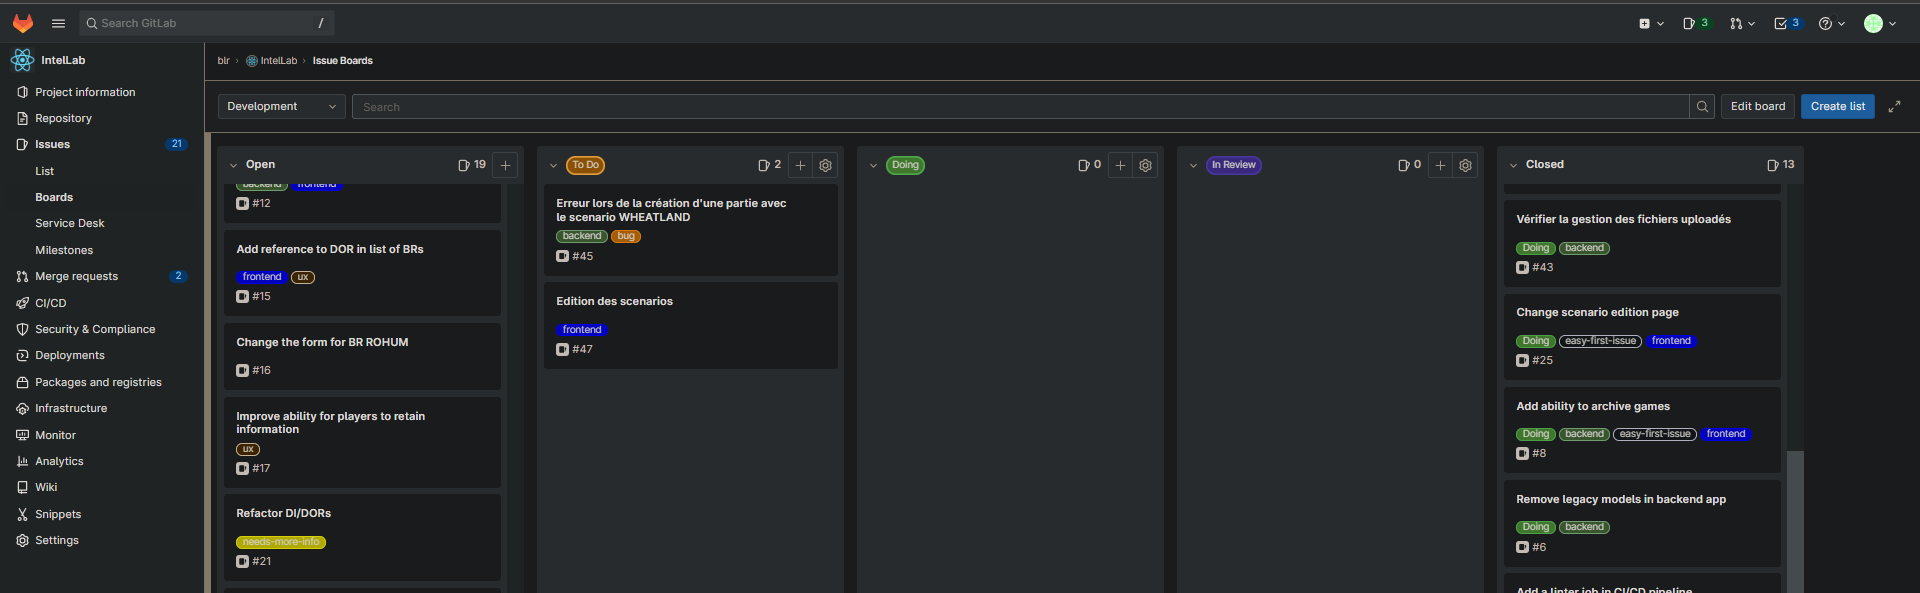
\includegraphics[width=\textwidth]{./images/gitlab_intellab.PNG}
	\caption[Planification des issues]{Planning issues - GitLab}\label{fig:gitlab_intellab}
\end{figure}

GitLab est une plateforme de gestion de code source basée sur Git qui permet aux équipes de développeurs de collaborer sur des projets de logiciels, de suivre les modifications du code source et de gérer des versions de code.
Elle offre des fonctionnalités pour la collaboration en temps réel, l'intégration continue et la livraison continue, la gestion de projet.


\subsection{Réalisation du projet}
IntelLab anciennement appelé \textbf{BLR (Battle Lab Rens)} a été initialement développé par un ancien ingénieur. Le BLR avait pour objectif la simulation exclusive des scénarios des services de renseignements militaires.
Dans l’optique de rendre l’application plus générique afin qu’elle s’adapte à d’autres types de scénarios autres que le renseignement militaire, le responsable informatique et moi avions procédé à la refonte complète de l’application en commençant par le changement de nom.


\subsubsection{Analyse du code existant et développement de la plateforme}

Avant de commencer le développement de l’application, nous avons effectué une analyse approfondie du code et de l’infrastructure du projet.
Ce qui nous a permis de mettre en place une logique de travail sur la restructuration de tout le projet.

Nous avons fait une refonte complète de l’application. La refonte avait pour but de restructurer le code afin de pouvoir poursuivre le développement de fonctionnalités nouvelles et de nouvelles fonctionnalités.
En parallèle, nous avons rédigé des tests unitaires et fonctionnelle pour garantir l'absence de détérioration dans la logique fonctionnelle de l'application après avoir effectué le remaniement du code que nous avons orchestré.


\subsubsection{Infrastructure des serveurs de développement et de production}

Il n'existait pas de serveur de développement sur lequel nous pouvions effectuer des tests de déploiement. Nous avons mis en place un serveur de développement qui sera par la suite la réplique parfaite du serveur de production.
Nous avons choisi d'utiliser Docker comme environnement d'exécution, installé sur un système d'exploitation Ubuntu Server.
La conteneurisation de nos serveurs nous offre une grande flexibilité dans la gestion des composants de notre application.
Ce serveur sert à vérifier le bon fonctionnement de l'application avant sa mise en production.

Les serveurs du backend, du frontend, du broker MQTT et de la base de données sont automatiquement installés dans l'environnement Docker des serveurs de développement et de production.
Cela est possible grâce au déploiement continu depuis GitLab que nous avons configuré, ce qui nous fait gagner énormément de temps pendant le déploiement.


\subsubsection{Description de l'infrastructure logicielle}

Cet environnement est développé en utilisant les technologies suivantes :

\begin{itemize}
	\item \textbf{Frontend} : ReactJS, gère l’interface utilisateur ;
	\item \textbf{Backend} :
	      \begin{itemize}
		      \item \textit{NodeJS} et \textit{ExpressJS} pour la partie serveur web ;
		      \item \textit{PostgreSQL} est le système de gestion de base de données ;
		      \item \textit{Sequelize} est utilisé pour les requêtes entre le serveur et la base de données ;
		      \item \textit{MQTT} : Il fournit une méthode de communication asynchrone de messages entre deux ou plusieurs appareils connectés à un réseau.
	      \end{itemize}
	\item \textbf{Infrastructure} :
	      \begin{itemize}
		      \item \textit{Docker} : Utilisé pour le déploiement de l’application sur les serveurs de test et de production ;
		      \item \textit{GitLab} : notre projet y est répertorié pour le travail collaboratif, les tests unitaires, les tests d’intégration, déploiement et intégration automatique.
	      \end{itemize}
	\item \textbf{Tests} :
	      \begin{itemize}
		      \item \textit{Vitest} : Outils de gestion des tests côté frontend ;
		      \item \textit{Jest} : Outils de gestion des tests côté backend.
	      \end{itemize}
\end{itemize}


\begin{figure}[h]
	\center%
	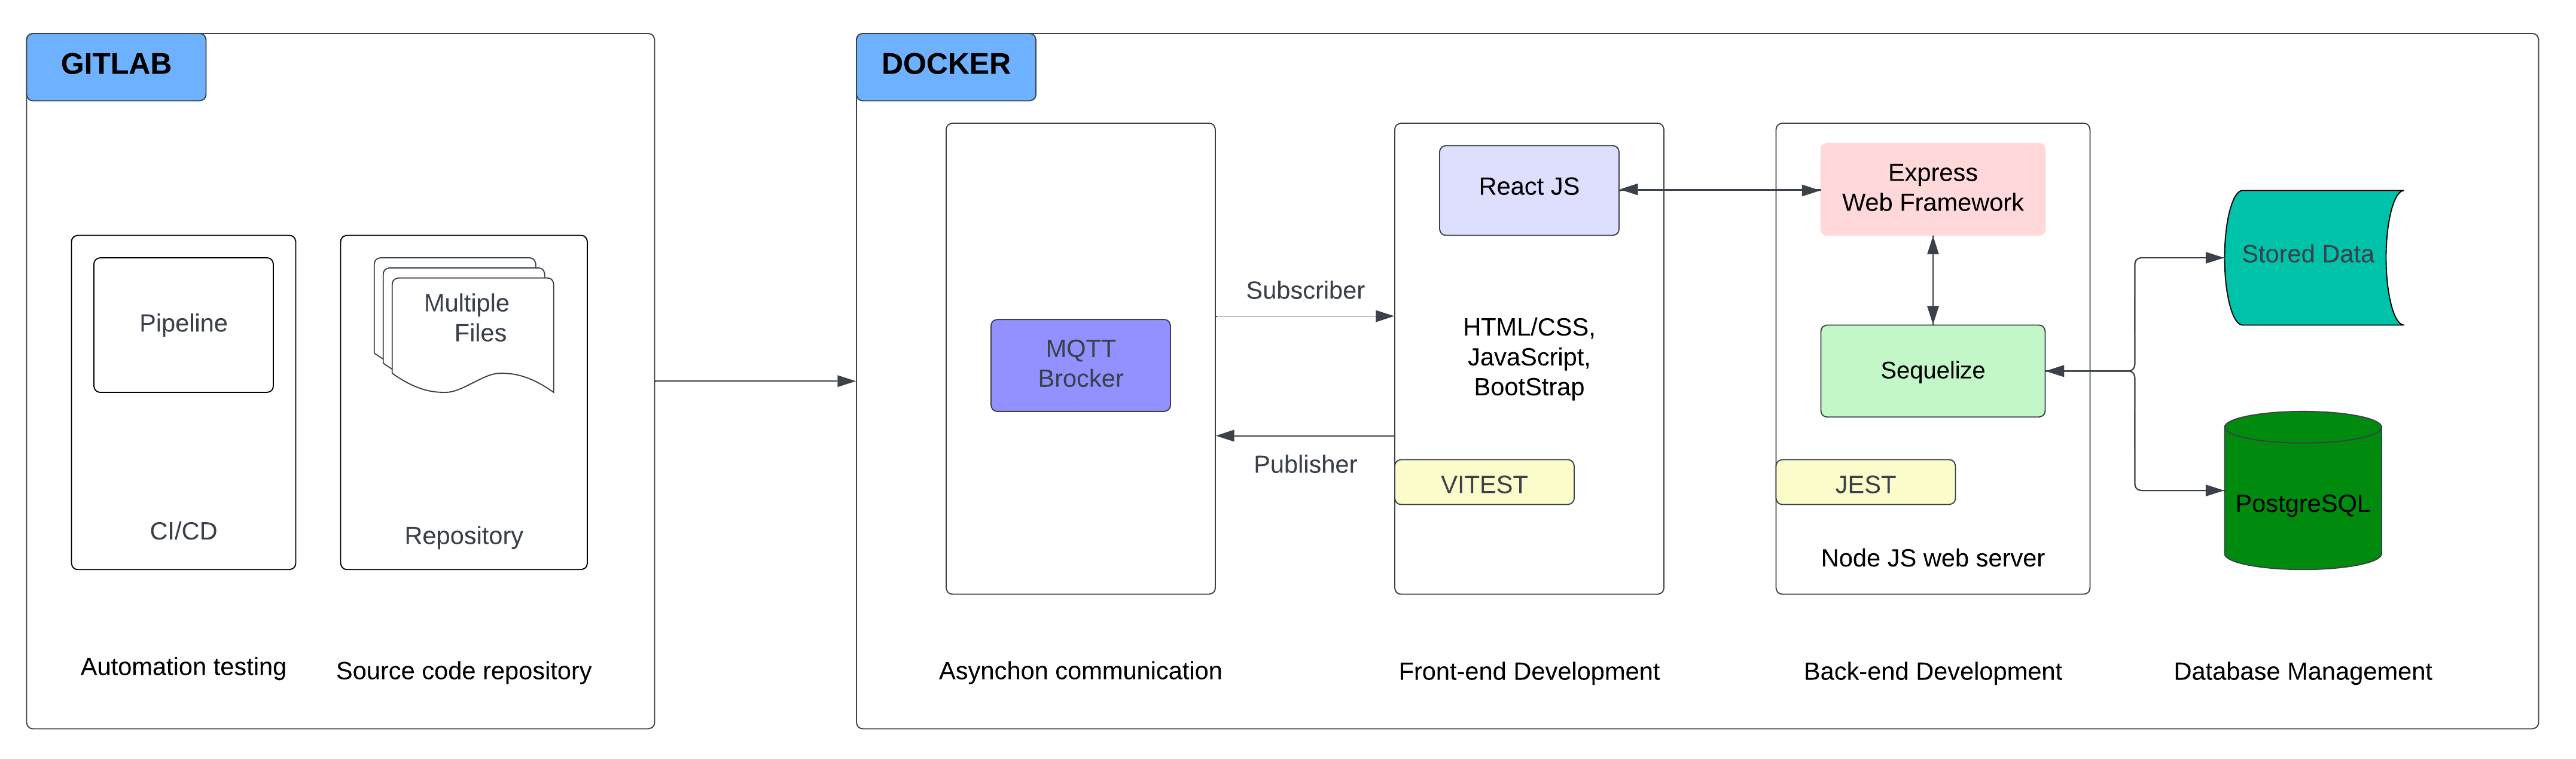
\includegraphics[width=\textwidth]{./images/architectur_intellab.png}
	\caption[Planification des issues]{Planning issues - GitLab}\label{fig:architectur_intellab}
\end{figure}


\subsection{Stratégie de tests}

En tant qu'environnement de simulation, formation et expérimentation, la fiabilité et la qualité d’IntelLab sont d'une importance capitale pour atteindre les objectifs visés par cette plateforme.
IntelLab est une application de recherche, donc nous n’avons pas les mêmes attentes ni besoins en termes de stratégie de tests.


\subsubsection{Objectifs et critères de tests}
Les tests sur IntelLab visent à assurer que l'application répond aux exigences fonctionnelles, en permettant des simulations réalistes et fiables des scénarios de renseignement.
Ils visent également à garantir la stabilité et la sécurité des données, à détecter et corriger les anomalies pendant les exercices, et à améliorer l'ergonomie et la convivialité de l'application pour une meilleure expérience utilisateur.


\subsubsection{Mise en place des outils de tests}

\begin{itemize}\addtolength{\itemsep}{-0.35\baselineskip}%
	\item \textbf{Outils de gestion des tests }: Nous utilisons l'outil de gestion des tests \textbf{vitest} coté frontend et \textbf{jest} coté backend pour suivre nos cas de test, les résultats des tests et les anomalies détectées.
	      \begin{figure}[h]
		      \center
		      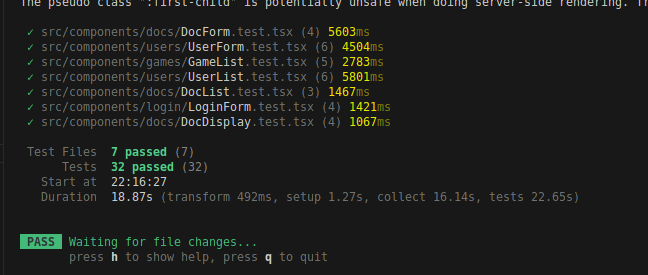
\includegraphics[scale=0.7]{./images/test_frontend_il.png}
		      \caption[Rapport test frontend avec VITEST]{Rapport tests avec VITEST}\label{fig:test_frontend_il}
	      \end{figure}
	\item \textbf{Outils d'automatisation des test} : Nous utilisons les pipelines de GitLab pour automatiser l'exécution des tests.
	      \begin{figure}[h]
		      \center
		      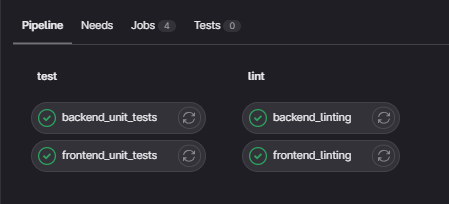
\includegraphics[scale=0.9]{./images/pipeline_tests.png}
		      \caption[pipeline des tests automatiques]{pipeline des tests automatiques}\label{fig:pipeline_tests}
	      \end{figure}
\end{itemize}


\subsubsection{Rédaction des procédures de tests}

\begin{itemize}
	\item \textbf{Scénarios de test} : Chaque scénario est accompagné de données de test spécifiques et de critères de succès clairement définis.
	\item \textbf{Procédures de test} : Nous documentons les procédures de test pour chaque type de test afin de garantir une exécution cohérente.
	\item \textbf{Critères d'acceptation} : Nous établissons des critères d'acceptation clairs pour chaque scénario de test, définissant ce qui est considéré comme un test réussi.
\end{itemize}

\begin{table}[h]
	\centering
	\begin{tabular}{|p{1.1cm}|p{3cm}|p{3cm}|p{4cm}|p{3cm}|}
		\hline
		\textbf{Menu Name} & \textbf{Description}                & \textbf{Test data}                & \textbf{Expected Output}                                     & \textbf{Actual Output}                                       \\ \hline
		Login              & should render a sign in button      & -                                 & Se connecter                                                 & Se connecter                                                 \\ \hline
		Login              & should display required helper text & Username: empty Password: Empty   & Le nom d'utilisateur est requis. Un mot de passe est requis. & Le nom d'utilisateur est requis. Un mot de passe est requis. \\ \hline
		Login              & should login user                   & Username: john Password: johnjohn & Connexion réussie                                            & Connexion réussie                                            \\ \hline
		Login              & should handle server errors         & Username: john Password: johnpass & Incorrect email or password                                  & Incorrect email or password                                  \\ \hline
	\end{tabular}
	\caption{Scénarios de test}
	\label{tab:test_scenarios}
\end{table}


\section{Projet IntelLab : Serveur de messagerie}

Ce projet a beaucoup de similitudes que celui de l'application Web. Nous allons ressortir quelques paries avec leur différences :


\subsection{Contexte du projet}
Le contexte initial de ce projet est pratiquement le même que celui de l'application web, la différence réside au niveau du type de scénario.
Ce projet permet la simulation des scénarios de types sécurité économique.
Ce type de scénario a exigé le développement d'une autre d'environnement car diffère du monde du renseignement militaire.
Cette plateforme est né du fait qu'on doit recréer un environnement d’entreprises telles que des startups ou des équipes de recherche.
Les objectifs la formation et la sensibilisation à la détection de signaux faibles précurseurs d’actions d’ingérence.


\subsection{Outils de gestion de projet}
Comme pour les autres projets, nous sommes une équipe de deux personnes, le responsable informatique et moi. Au vu de cela, nous avons toujours adopté la méthodologie agile car cela nous permet de gérer efficacement nos ressources limitées, de nous adapter rapidement aux changements de priorités, et de livrer des fonctionnalités clés du serveur de messagerie de manière itérative et continue, en garantissant une meilleure réactivité aux besoins des utilisateurs finaux.


\subsubsection{Planification des tâches}
Comme pour l'autre projet, nous avons centralisé la gestion de ce projet sur la plateforme GitLab.
La description des taches, la gestion du code, collaboration en temps réel, l’intégration continue et le déploiement automatique, toutes ses fonctionnalités sont gérées sur la plateforme GitLab.


\begin{figure}[h]
	\center
	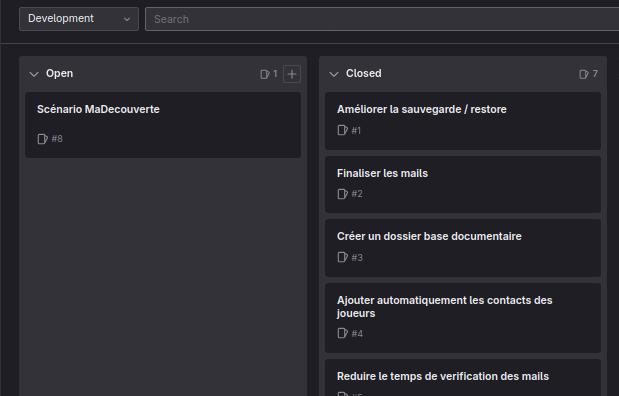
\includegraphics[width=0.6\textwidth]{./images/gitlab_mpc.png}
	\caption[Planification des issues MPC]{Planning issues MPC - GitLab}\label{fig:gitlab_mpc}
\end{figure}





































% --------------------------------------------------------------------------
\section{Projet Détection et reconnaissance de véhicules militaires sur des images et vidéos (DetReco)}

\subsection{Context du projet DetReco}

Le projet DetReco s'inscrit dans une collaboration stratégique entre l'équipe STARS du centre de Sophia-Antipolis, la Direction Générale de l'Armement (DGA), et le département Défense et Sécurité de l'Inria. Ce projet a pour objectif de mener une étude approfondie de l'état de l'art des algorithmes appliqués à la détection et à la reconnaissance, en temps quasi réel, de véhicules militaires sur des images et vidéos.



\section{Analyse}

\section{Résultats obtenus}







% \subsection{Inria : métiers et chiffres clés.}



% \begin{itemize}
% 	\item The individual \index{Entries}{entries} are indicated with a black dot, a so-called bullet.
% 	\item The text in the entries may be of any length.
% \end{itemize}

% \begin{theorem}\label{theo1}
% 	Soit $n$ un entier naturel. Si $n$ est premier alors il n'est divisible que par 1 et par lui-même.
% \end{theorem}

% \begin{proof}
% 	Here is my proof.
% \end{proof}

% \begin{definition}\label{def1}
% 	Soit $A$ une courbe...
% \end{definition}

% Ici, il s'agit de l'utilisation de TB %\nomenclature[TB]{TB}{Très Bien} qui consiste à parler Très Bien. 
% \gls{abc} et \gls{efg} sont des acronyms et des abbréviations... La méthode \gls{svm} est également couramment utilisée.

% \begin{exemple}\label{exo1}
% 	On considère le cas particulier...
% \end{exemple}